\chapter{Úložiště velkých dat}\label{kap:storage}
S~přibývajícím množstvím moderních technologií a odvětví (například IoT -- Internet of Things) vznikají nové problémy s~množstvím dat, které generují. Ať už jde o~záznamy o~uživatelích sociálních sítí, souřadnice polohy osob či vozidel sbíraných chytrými telefony, historii nákupů na internetovém obchodě nebo měření ze senzorů, je potřeba tyto informace  uchovávat a zároveň musí být rychle a snadno dostupné pro zpracování. Jelikož se může jednat o~obrovské množství dat, nároky na tyto systémy jsou velmi vysoké. Pro představu o~jaké množství dat může jít si vezměme například službu Timeline od společnosti Google. Při povolení této služby chytrý mobilní telefon snímá polohu přístroje a vlastník připojeného účtu má zpětně přehled o~svém pohybu a činnostech. Během dne může být takto vygenerováno od pár desítek po několik tisíc záznamů, které je potřeba uložit a v~případě potřeby zpřístupnit. Samo o~sobě se nejedná o~velké množství dat, ale když vezmeme v~úvahu množství lidí využívající chytrý telefon, mluvíme zde o~sta milionech záznamů denně. 

K~ukládání takového objemu dat se využívají mimo jiné distribuované souborové systémy, cloudové nástroje či specializované databázové systémy. Tato kapitola je věnována různým typům úložišť pro tato data a je zaměřena na řešení určené pro ukládání hodnot získaných během měření různých senzorů. U~tohoto typu dat je nejdůležitějším údajem každého záznamu kombinace času měření a naměřené hodnoty. Kapitola má tedy za cíl seznámit čtenáře s~technologiemi, které se často využívají pro ukládání velkých dat a s~vysvětlením jejich principů.

\section{NoSQL}
Jedná se o~nerelační datový model podporující distribuovanou architekturu a umožňující zpracování velkého množství dat - až petabajty dat za den. Oproti relačnímu modelu obětuje přílišnou komplexnost způsobující striktní zajištění pravidel ACID (Atomicity, Consistency, Isolation, Durability) tzn. atomičnost transakcí, konzistenci dat, neovlivnění souběžných transakcí a ochrana proti ztrátě transakcí. Tato ztráta komplexnosti sice umožňuje inkonzistenci a nepřesnost, to ale kompenzuje vysokou propustností a škálovatelností. Tento model je proto vhodný pro data, u~kterých nejsou drobné nepřesnosti problematické a je potřeba jich zpracovávat obrovské množství, jako například u~sledování dat ze senzorů či monitorování sítě a podobně. Tento model je proto naprosto nevhodný k~uchování dat vyžadující konzistenci (například bankovní transakce), kde i ztráta jednoho záznamu může znamenat katastrofu. Ztráta záznamu ale není velkým problémem třeba u~monitorování síťového vytížení, kde se stejně agreguje obrovské množství hodnot a nedojde proto k~velkému ovlivnění výsledku. Možnost nezajistit konzistenci proto dovoluje právě povaha dat, pro která jsou úložiště využívající tento model určena \cite{NoSQL}.

\section{Hadoop Distributed File System} \label{HDFS}
Hadoop Distributed File System (dále jen HDFS) je součástí volně dostupného projektu Apache Hadoop. Jedná se o~distribuovaný souborový systém poskytující vysokou propustnost dat a toleranci poruch. V~této sekci a jejích podsekcích byly informace čerpány z~dokumentace projektu HDFS\cite{HDFSDoku}.

\subsection{Architektura HDFS}
HDFS využívá architekturu master/slave a je distribuovaný, tudíž využívá více datových uzlů. Samotné blokové schéma systému je zobrazena na obrázku \ref{pic:hdfs_architecture}. Datové uzly se starají o~samotné úložiště. Většinou je umístěn právě jeden datový uzel na fyzickém serveru. Umístění více instancí uzlu na jeden fyzický server nepřidává žádné výhody. HDFS umožňuje uživateli ukládat data do souborů, které jsou následně rozděleny na bloky a ty jsou distribuovány mezi několik datových uzlů. Datové uzly se také starají o~veškeré operace s~bloky - vytváření, mazání, replikace, čtení a zápis.

\begin{figure}[h]
  \centering
  \scalebox{0.50}{
        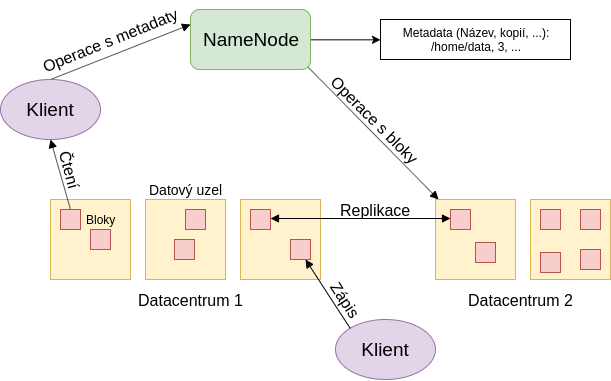
\includegraphics{obrazky-figures/HDFSarchitecture.png}
    }
  \caption{Schéma architektury HDFS \cite{HDFSDoku}.}\label{pic:hdfs_architecture}
\end{figure}

Všechny bloky souboru mají stejnou velikost - vyjma posledního. Jednotlivé bloky jsou replikovány napříč uzly a tím se dosahuje tolerance poruch uzlů. Velikost bloků a počty jejich kopií (replikační faktor) jsou nastavitelné pro každý soubor zvlášť a tyto hodnoty jsou udržované v~metadatech. Soubor v~HDFS lze zapsat pouze jednou a jedním uživatelem. 

Datové uzly spravuje \textit{NameNode}. Jedná se o hlavní server, který se stará o~hierarchii souborového systému, metadata a upravuje přístup klientům. Jakoukoliv změnu umístění či vlastností (například replikační faktor, název, id) zaznamenává do logu a mění v~metadatech. \textit{NameNode} se stará o~veškerá rozhodnutí týkající se replikace bloků. Od každého datového uzlu periodicky dostává upozornění indikující správnou funkčnost (takzvaný \textit{Heartbeat}) a seznam jednotlivých uložených bloků. 


\subsection{HBase} \label{Hbase}
HBase je taktéž součást Apache Hadoop a jedná se o~sloupcově orientovaný nerelační databázový systém operující nad HDFS (viz \ref{HDFS}). HBase je nástroj vhodný pro zpracovávání dat v~reálném čase, náhodný přístup k~velkému množství dat a je lineárně škálovatelný. Nepodporuje strukturované dotazy jako SQL. Systém lze lineárně škálovat. Každá tabulka musí obsahovat primární klíč a k~uloženým datům lze přistupovat pouze přes tento primární klíč \cite{HBase}.

\section{Google BigTable}\label{sec:bigtable}
Jedná se o~distribuovaný systém využívaný pro ukládání dat a je navržen tak, aby byl schopný pracovat s~ohromným množstvím dat na velkém počtu serverů. V~této sekci čerpám informace z~\cite{BigTable}.

BigTable je multidimenzionální tříděná mapa. Základní jednotkou je netypovaný řetězec znaků, který je interně uložený v~blocích ve tříděných tabulkách řetězců znaků zvaných SSTable. Tyto bloky jsou dostatečně malé na to, aby je bylo možné nahrát do operační paměti (typicky 64 kB). Na konci každé tabulky je uložen index, který je nahrán do paměti při otevření tabulky. BigTable indexuje podle řetězce znaků, přesněji podle řádku, sloupce a verze (většinou se jedná o~časovou značku). Záznamy mají lexikografické uspořádání. Tabulky jsou ukládány po blocích zvaných \textit{tablet} podle rozsahu a pokud tento blok překročí určitou velikost, je rozdělen na dva tablety (bloky jsou typicky 100-200 MB velké). Schéma tabletu je možné vidět na obrázku číslo \ref{pic:tablet}. Každý záznam obsahuje verzi, která je záznamům přidělována automaticky jako časová značka aktuálního času při zápisu, tím se předchází možným kolizím hodnot. Verzi lze přidělovat i z~klientské aplikace, která BigTable využívá, ale potom je na klientské aplikaci, aby zajistila unikátnost záznamů. Verze záznamu je využívána pro mazání starých a neaktuálních hodnot. Klient může specifikovat kolik záznamů nebo jaký časový úsek do minulosti má být uchováván.

Samotný systém obsahuje dva typy serverů - master a tablet server. Master server je puštěn pouze v~jedné instanci a stará se o~rozdělení tabletů tablet serverům, detekci expirace tablet serverů, vyvažování zatížení, zálohy a změny schémat systému. Tablet servery se starají o~tablety, zápis, čtení a rozdělení tabletů při překonání určité velikosti. Klientské aplikace komunikují přímo s~tablet servery. Ke správě záloh se využívá služba zvaná \textit{Chubby}. Pro zjištění polohy uložených dat slouží tříúrovňový B-strom, obsahující metadata o~tabletech. 

\begin{figure}[h]
  \centering
  \scalebox{0.43}{
        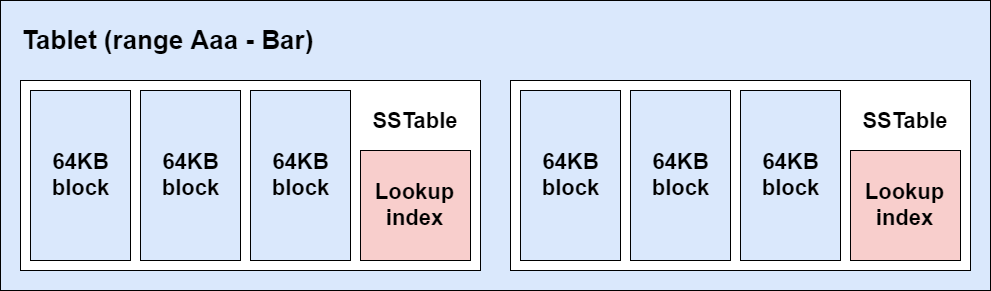
\includegraphics{obrazky-figures/bigtable_tablet.png}
    }
  \caption{Schéma tabletu \cite{BigTableTablet}.}\label{pic:tablet}
\end{figure}

\section{Time-series databáze}
Časová databáze (lépe známé pod anglickým názvem \textit{time-series database}) je speciálním typem databáze určené a optimalizované pro zaznamenávání měření obsahující časovou značku. Tyto databáze se využívají ve finančním sektoru (historie stavu akcií pro predikce jejich budoucího vývoje), telekomunikacích (informace o~stavu a využití sítí), nebo při monitoringu datových center (monitorování teploty, využití procesorů, poruch) či průmyslových strojů.

Jak už tedy název napovídá, pracují s~časovou značkou, která se vyskytuje u~každého záznamu, a je vždy primárním klíčem nebo alespoň jeho součástí. Časová databáze typicky obsahuje datové body, které představují měření v~daném čase.  Oproti relačním databázím se téměř nepočítá s~využitím funkcí pro aktualizaci (UPDATE) či mazání (DELETE) hodnot a dotazy (SELECT) jsou velmi specifické. Složité složené dotazy plné podmínek nejsou časté pro data tohoto typu a nejčastějším typem dotazů je získání určitého časového okna měřených dat, a to co nejefektivněji. Právě na tyto dotazy jsou časové databáze optimalizovány\cite{time-series-paper}. 

Časové databáze jsou obvykle postaveny nad distribuovanými souborovými systémy, jako jsou HDFS či Bigtable popsané dříve v~této kapitole, a s~jejich pomocí dosahují vysoké rychlosti čtení a zápisu hodnot a škálovatelnosti systému.

Kromě času obsahují časové databáze jako OpenTSDB nebo InfluxDB dva další typy hodnot - značky (\textit{tag}) a datová políčka (\textit{field}). Databáze následně zajišťuje unikátnost záznamu pomocí primárního klíče složeného z~kombinace času, značek a měřené hodnoty. Záznamy jsou následně ukládány v~balících podle značek a v~těchto balících jsou seřazeny podle času. Tento přístup zrychluje možnost agregace uložených hodnot \cite{time-series-book}.

\subsection{Řádkově/sloupcově orientované ukládání}
Databáze využívají k~ukládání dat dva způsoby - jsou sloupcově nebo řádkově orientované. Řádkově orientovaná metoda je používaná relačními databázemi. Ukládá a získává data po řádcích. Tento způsob uložení není efektivní pro agregaci a analýzu většího množství hodnot a dosahuje horší úrovně komprese dat než ukládání po sloupcích. Čtení a zápis je ale snazší. Sloupcově orientované databáze oproti tomu ukládají a získávají data po sloupcích. Příkladem je HBase, která je základem některých časových databází. Touto metodou lze dosáhnout rychlé agregace velkého množstvím hodnot a umožňuje vysokou úroveň komprese díky podobnosti hodnot, které jsou za sebou uložené. Přestože sloupcově orientované databáze dominují úložištím velkých dat, lze nalézt i databáze které kombinují oba způsoby, jako je TimescaleDB \cite{rowColumn}.

\subsection{Zástupci}
S~rostoucí potřebou zpracování a uložení dat z~měření se v~posledních letech rozšířil počet různých časových databází. Nejedná se již jen o~obecné implementace jak tomu bylo dříve, ale i o~databáze určené ke specifickým účelům, na míru vyvinutým potřebám firem, jako je Facebook či Google. Nejznámější a nejpoužívanější time-series databáze jsou následující:

\subsubsection*{OpenTSDB}
Jedná se o~škálovatelnou volně dostupnou časovou databázi pracující nad HBase (popsanou v~\ref{Hbase}) či Google Bigtable (popsaný v~sekci \ref{sec:bigtable}). OpenTSDB nabízí rozhraní pro zápis a čtení a stará se o~veškeré operace související se správou HBase. Data lze získat v~grafické formě či ve formě souboru ve formátu json.

Jak je vidět na obrázku \ref{pic:OpenTSDB}, OpenTSDB je vlastně několik samostatných TSD instancí, které zastřešují přístup k~úložišti a starají se o~veškerou komunikaci. Uživatel tedy přistupuje k~datům pouze s~pomocí poskytnutého rozhraní. Databáze je optimalizovaná pro rychlou agregaci hodnot. Čas je uložen ve formě unixové časové značky a hodnoty jsou 64bitová celá či desetinná čísla. Přístup k~datům je možný pomocí vestavěného grafického rozhraní či přes HTTP rozhraní \cite{TSDBdoku}.

\begin{figure}[!tbp]
  \centering
  \begin{minipage}[b]{0.45\textwidth}
    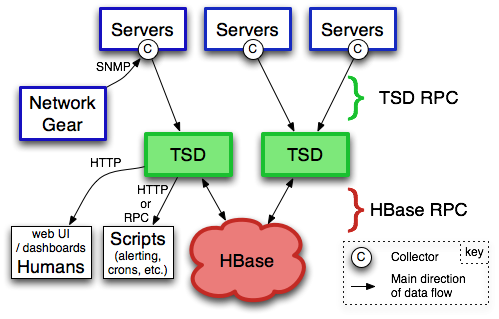
\includegraphics[width=\textwidth]{obrazky-figures/tsdb-architecture.png}
    \caption{Architektura OpenTSDB \cite{TSDBdoku}.}
    \label{pic:OpenTSDB}
  \end{minipage}
  \hfill
  \begin{minipage}[b]{0.45\textwidth}
    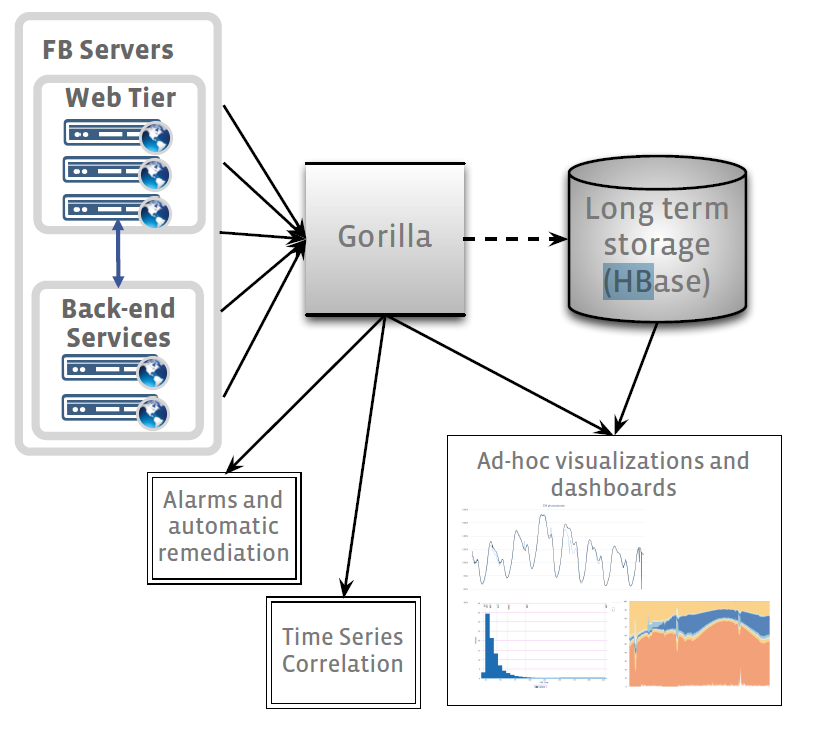
\includegraphics[width=\textwidth]{obrazky-figures/gorilla.PNG}
    \caption{Schéma využití databáze Gorilla \cite{gorilla}.}
    \label{pic:gorilla}
  \end{minipage}
\end{figure}

\subsubsection*{InfluxDB}
Informace o~InfluxDB byly čerpány z~\cite{Influx}. Databáze InfluxDB byla vytvořena již od základu jako časová a je k~dispozici volně dostupná i v~komerční verzi. Jedná se o~NoSQL databázi implementovanou v~jazyce Go. Komerční verze nabízí dodatečnou funkcionalitu nutnou pro nasazení ve větším měřítku - například možnost využití instancí na více serverech či pokročilé monitorování. Jedná se o~nejpopulárnější časovou databázi. InfluxDB se skládá z databází, které obsahují jednotlivé hodnoty uspořádané podle měření (\textit{Measurement}). Měření se dá přirovnat k~tabulkám. Záznam obsahuje název měření, set tagů podle kterých se indexuje, set hodnot podle kterých se neindexuje a časovou značku v~přesnosti na nanosekundy. Počet tagů není omezený na rozdíl od OpenTSDB. InfluxDB poskytuje jazyk pro dotazy podobný SQL dotazům. Pro každé měření lze nastavit jak dlouho a v~kolika kopiích mají být hodnoty uchovány. InfluxDB využívá svůj vlastní úložný engine zvaný TSMT (Time Structured Merge Tree). Databáze ukládá data po blocích zvaných \textit{shard}, které jsou organizovány podle nastavení životnosti dat do časových úseků. Základní časový úsek pro životnost dat kratší než dva dny je jedna hodina, a pro životnost delší než 6 měsíců je časový úsek jednoho bloku 7 dní.

\begin{figure}%[h]
  \centering
  \scalebox{0.43}{
        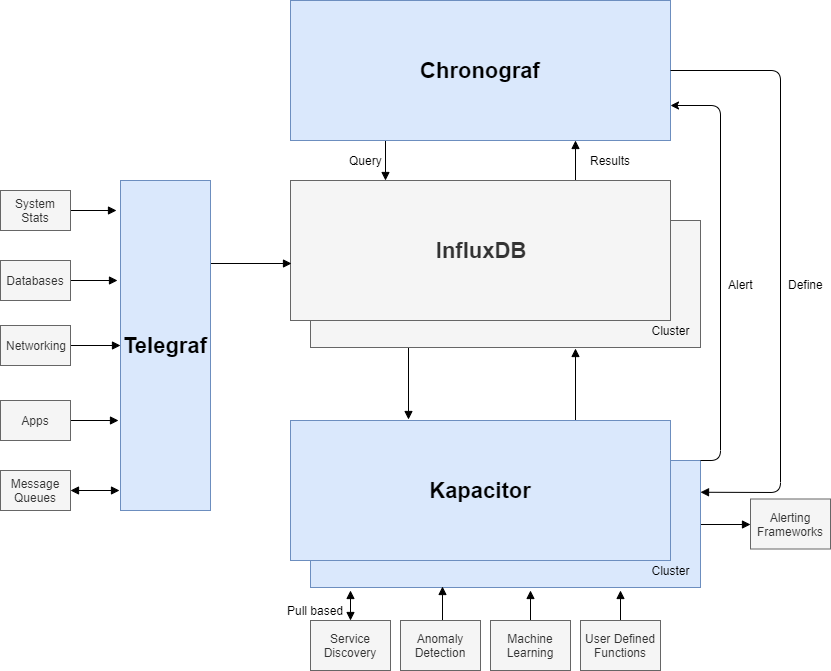
\includegraphics{obrazky-figures/influx.png}
    }
  \caption{Schéma platformy Tick \cite{Influx}.}\label{pic:tick}
\end{figure}

K~datům lze přistupovat přes HTTP a UDP komunikační rozhraní, přes konzoli podobně jako u~MySQL či přes webovou aplikaci Chronograf. InfluxDB a Chronograf jsou součástí platformy TICK. Součástí této platformy je i modul Telegraf, který slouží k~monitorování serverů, na kterých je spuštěn InfluxDB, a engine pro zpracovávání dat v~reálném čase Kapacitor. 
Na obrázku číslo \ref{pic:tick} je znázorněno schéma platformy TICK s~databází InfluxDB ve svém jádru.

\subsubsection*{Gorilla} \label{sec:gorilla}
Technické informace této části pochází z~\cite{gorilla}. Gorilla je \textit{in-memory} databáze (data jsou uložena v operační paměti) vytvořená firmou Facebook, která slouží pro monitorování dat zapisovaných do HBase databáze. Vizualizované využití této databáze je možné vidět na obrázku \ref{pic:gorilla}. Bod uložený v~databázi obsahuje klíč ve formě posloupnosti znaků, 64bitové časové značky a desetinného čísla obsahujícího hodnotu. Jelikož se jedná o~\textit{in-memory} databázi, která funguje jako mezipaměť pro dlouhodobější uchování dat na discích, jsou hodnoty udržovány po omezenou dobu. Množství bodů je ale natolik velké, že požadavky na paměť by byly v~řádech desítek terabajtů, proto databáze využívá kompresních algoritmů popsaných v~\ref{sec:delta} a \ref{sec:xor}. Tento algoritmus umožňuje průměrnou kompresi 16 bajtů na 1,37 bajtu. Gorilla se také od ostatních časových databází odlišuje svou úzkou specializací na monitorování systémů v~reálném čase. Databáze má za cíl co nejrychleji odhalovat chyby v~interních systémech. Databáze musí být schopná bez výpadku přijímat a zapisovat velké množství bodů i za cenu dočasné nedostupnosti pro čtení nebo ztráty starších bodů. Proto není kladen důraz na jednotlivé body, ale na agregované analýzy. Gorilla je distribuovaná mezi několik regionů bez zajištění konzistence a dotazy jsou směrovány na nejbližší datová centra. To umožňuje tolerovat výpadek celého regionu.

Hodnoty jsou uloženy ve formě \textit{TSMap}. Ta je složena z~vektorů sdílených ukazatelů na časové série a mapy obsahující dvojice název série a ukazatel na její umístění v~paměti. Při smazání série nejsou data smazána, ale paměť je pouze označena pro znovupoužití. Výlučný přístup k~datům zajišťuje zámek na \textit{TSmap} a 1-bajtový zámek s~aktivním čekáním na každé časové sérii.

\subsubsection*{TimescaleDB}
Zdrojem informací o~architektuře TimescaleDB je \cite{TimescaleDoku}. Oproti výše zmíněným databázím je TimescaleDB založená na relačním databázovém modelu využívající PostgreSQL. TimescaleDB je zaměřená na lepší paralelní zpracování a škálování nejen na více uzlů, ale i na jednom samotném uzlu. Je ale nutno zmínit, že v~době psaní této práce bylo škálování na více uzlů stále ve fázi vývoje. Oproti databázím, jako je InfluxDB, nerozděluje data do bloků o~jedné dimenzi (v~případě zmíněné databáze InfluxDB podle času), které lze následně ukládat na různých uzlech, ale do bloků o~více dimenzích, ke kterým uživatel přistupuje přes struktury zvané \textit{hypertable}. Data jsou rozdělena primárně podle času a dále podle klíče, kterým může být například identifikátor. Právě toto rozdělení umožňuje škálovat databázi i na jednom uzlu. \textit{Hypertable} je abstrakce tabulky, jak je známá například z~MySQL. Dotazy či jiné interakce s~databází se provádí nad těmito tabulkami. Jedná se tedy virtuálně o~standardní schéma obsahující sloupce. Minimálně jeden sloupec musí obsahovat časovou značku. Další sloupce obsahující klíče, podle kterých se provádí rozdělení dat, jsou volitelné. Jednotlivé bloky jsou implementovány pomocí PostgreSQL tabulek a obsahují určitý časový a prostorový interval, který závisí na schématu. Data se nepřekrývají a to snižuje počet přístupů k~jednotlivým fyzickým tabulkám. Data jsou v~databázi uložena jak v~řádkovém, tak ve sloupcovém formátu. Jakmile jsou data dostatečně stará, jsou komprimovaná z~řádkového formátu do sloupcového. Tato architektura umožňuje TimescaleDB mnohem vyšší propustnost bodů pro zápis na jednom uzlu, než konkurenční InfluxDB. Porovnání mezi InfluxDB a TimescaleDB v~počtu zapsaných bodů na jednom uzlu za vteřinu je možné vidět na obrázku \ref{pic:timescaleComparisson}.

\begin{figure}[h]
  \centering
  \scalebox{0.40}{
        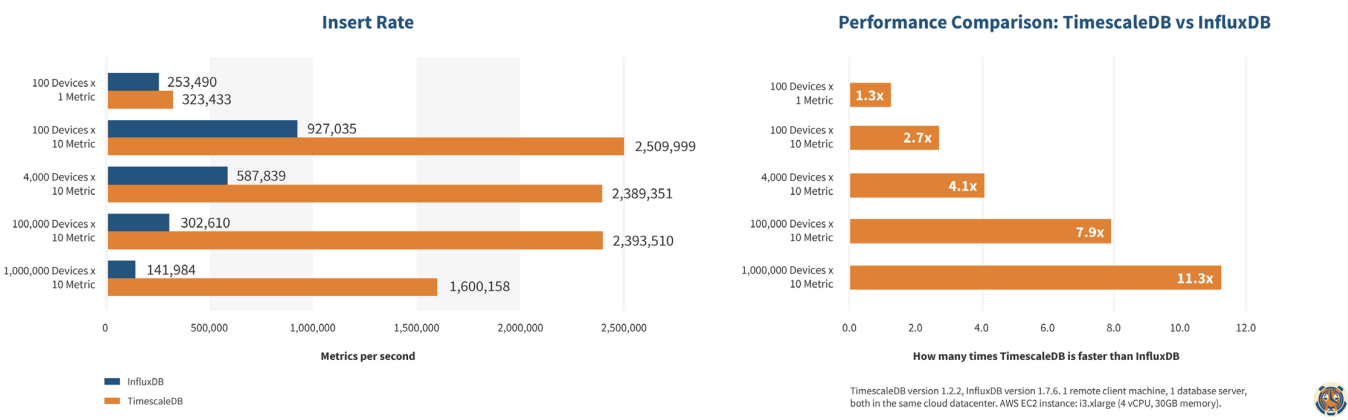
\includegraphics{obrazky-figures/db_comparisson.PNG}
    }
  \caption{Porovnání InfluxDB a TimescaleDB v~počtu vložených bodů za vteřinu na jednom uzlu \cite{InfluxVsTimescale}.}\label{pic:timescaleComparisson}
\end{figure}

%\section{Rozhraní pro komunikaci s úložišti}